% Chapter Template

\chapter{Applying atomistic and coarse-grained simulation to reflectometry analysis} % Main chapter title

\label{reflectometry2} % Change X to a consecutive number; for referencing this chapter elsewhere, use \ref{ChapterX}

%----------------------------------------------------------------------------------------
%	SECTION 1
%----------------------------------------------------------------------------------------

\section*{Abstract}
The use of molecular simulation to aid in the analysis of neutron reflectometry measurements has become commonplace.
However, reflectometry is a tool to probe large-scale structures, and therefore the use of all-atom simulation may be irrelevant.
This work presents the first direct comparison between the reflectometry profiles obtained from different all-atom and coarse-grained molecular dynamics simulations and the reflectometry profiles from a chemically-consistent layer-based modelling method.
We find that systematic limitations reduce the efficacy of the MARTINI potential model, while the Berger united-atom and Slipids all-atom potential models agree similarly well with the experimental data.
The chemically-consistent layer model gives the best agreement, however, the higher resolution simulation-dependent methods produce an agreement that is comparable.

\section*{Context}
This chapter builds on the previous chapter, by using the traditional, highly coarse-grained, chemically-consistent layer model as a point of comparison with classical molecular simulations of a variety of simulation grain-size, from the coarse-grained MARTINI potential model, to the all-atom Slipids.
Therefore, the chapter applies significantly more constraints on the system, however, the constraints are built on substantial underlying chemistry, given there grounding in the potential models.
It is hoped that this work will provide as an advisory document to those interested in applying classical simulation to the analysis of their neutron reflectometry experiments.
Furthermore, the simulations are used to advise on ways that the chemically-consistent models may be improved in the future.
It is noted again that the focus of this chapter is the methodological developments, rather than the particular chemical system to which they are applied.

\subsection*{Publications}
Parts of this work have been published in , a copy of the publication may be found in Appendix~\ref{papers}.

\pagebreak
\section{Introduction}
The use of a traditional, layer-based model approach\footnote{As is outlined in Chapter~\ref{reflectometry1}.} is a powerful tool to understand the structure of complex systems such as biomimetic bacterial membranes\autocite{barker_neutron_2016} and polymeric energy materials.\autocite{khodakarimi_x-ray_2016}
These layers structures are typically defined by the underlying chemistry of the system.
However, there has been growing interest in the use of MD simulations to inform the development of these layer structures.
This is due to the fact that the equilibrium structures for soft matter interfaces, that are often of interest in reflectometry studies, are accessible on all-atom simulation timescales.\autocite{scoppola_combining_2018}
However, there has been no work that directly compares different levels of simulation coarse-graining in order to assess the required resolution for the accurate reproduction of a given NR profile.

Simulation-driven multi-modal analysis has been applied previously, either by the calculation of the SLD profile from the simulation by the full determination of the reflectometry profile.
In the former case, the calculated SLD profile may be compared with the SLD profile determined from the use of a traditional analysis method.
Bobone \emph{et al.} used such a method to study the antimicrobial peptide trichogin GA-IV within a supported phospholipid bilayer.\autocite{bobone_membrane_2013}
A four-layer model consisting of the hydrated \ce{SiO2} layer, an inner phospholipid head-region, a phospholipid tail-region, and an outer phospholipid head region was used in the Abel\`{e}s matrix formalism.
The SLD profile from the MD simulations agreed well with that fitted to the reflectometry data from the layer model.

The reflectometry profile was determined explicitly from the classical simulation in the works of Miller \emph{et al.} and Anderson and Wilson.\autocite{miller_monte_2003,anderson_molecular_2004}
In these studies, an amphiphilic polymer at the oil-water interface was simulated by Monte Carlo and MD respectively, and the NR profile was found by splitting the simulation cell into a series of small layers and treating these layers with the Abel\`{e}s formalism.
There was good agreement between the experimental and calculated reflectometry, for low interfacial coverages of the polymer.
Another study that has made a direct comparison between the atomistic simulation-derived reflectometry data and those measured experimentally includes that of Darr\'{e} \emph{et al.}.\autocite{darre_molecular_2015}
In this work, NeutronRefTools was developed to produce the NR profile from an MD simulation.
The particular system studied was a supported DMPC phospholipid bilayer, with good agreement found between the simulation-derived profile and the associated experimental measurements.
However, the nature of the support required that a correction for the head group hydration be imposed to achieve this agreement.

Koutsioubas used the MARTINI coarse-grained representation of a DPPC phospholipid bilayer to compare with experimental reflectometry.\autocite{koutsioubas_combined_2016}
This work shows that the parameterisation of the MARTINI water bead was extremely important in the reproduction of the reflectometry data, as the non-polarisable water bead would freeze into crystalline sheets resulting in artefacts in the reflectometry profiles calculated.
The work of Hughes \emph{et al.} studied, again, a DPPC phospholipid bilayer system,\autocite{hughes_interpretation_2016} albeit an all-atom representation, that was compared with a supported DPPC phospholipid bilayer system measured with polarised NR.
The SLD profile found from MD simulation was varied to better fit the experimental measurement, resulting in good agreement.
Additionally, the ability to vary the SLD profile was used to remove an anomalous difference present in the SLD, that arose when the MD simulations were merged with an Abel\`{e}s layer model.
This was done to account for regions present in the experiment that were not modelled explicitly.

In all the examples discussed so far, there is no direct comparison between the reflectometry profile determined from simulation and that from the application of a traditional modelling approach.
Indeed, the only example,\footnote{To the author's knowledge.} where a direct comparison was drawn is the work of Dabkowska \emph{et al.}.\autocite{dabkowska_modulation_2014}
This work compares the reflectometry profile from a DPPC monolayer at the air-water interface containing dimethyl sulfoxide molecules with a similar MD simulation using the CHARMM potential model.
The use of multimodal analysis allowed the determination of the position and orientation of dimethyl sulfoxide molecules at a particular region within the monolayer.

The previously mentioned work of Koutsioubas involved the use of the MARTINI coarse-grained potential model to simulate the DPPC bilayer system.\autocite{koutsioubas_combined_2016}
The use of atomistic simulation for soft matter systems, such as a phospholipid bilayer, is undesirable as this requires a huge number of atoms to be simulated, due to the large lengths scales involved.
The purpose of simulation coarse-graining is to reduce the number of particles over which the forces must be integrated, additionally, by removing the higher frequency bond vibrations, the simulation timestep can also be increased.\autocite{pluhackova_biomembranes_2015}
Together, these two factors enable an increase in both simulation size and length.
The use of the MARTINI 4-to-1 coarse-grained and the Berger united atom\footnote{Where hydrogen atoms are integrated into the heavier atoms to which they are bound.} potential models are particularly pertinent for the application to phospholipid simulations as both were developed with this specific application in mind.\autocite{marrink_martini_2007,berger_molecular_1997}

The MARTINI potential model involves integrating the interactions of every four heavy atoms\footnote{Larger than hydrogen.} into beads of different chemical nature.
This potential model attempts to simplify the interactions of phospholipid and protein molecules significantly by allowing for only eighteen particle types, defined by their polarity, charge, and hydrogen-bond acceptor/donor character, which are discussed in detail in the work of Marrink \emph{et al.}\autocite{marrink_martini_2007}
This coarse-grained potential model was initially developed for the simulation of a phospholipid bilayer, and proteins held within and therefore is parameterised well under these conditions.
It has successfully been used to simulate a wide range of systems, such as DNA nucleotides,\autocite{uusitalo_martini_2015} the micellisation of zwitterionic and nonionic surfactants,\autocite{sanders_micellization_2010} and the self-assembly of ionic surfactants.\autocite{wang_coarse-grained_2015}

Increasing the simulation resolution gives an united-atom potential model, where all of the hydrogen atoms are integrated into the heavier atoms to which they are bound.
One of the most popular united-atom potential models for phospholipid simulations is that developed by Berger \emph{et al.}.\autocite{berger_molecular_1997}
The Berger parameters were optimised to reproduce phospholipid density and area per phospholipid, the latter of which is often an important parameter for the understanding of reflectometry profiles.
Since its inception, this potential model has proven one of the most commonly used and resilient sets of phospholipid parameters, with the original paper being cited 1500 times at the time of writing.
Applications of this potential model have mostly been focussed on the simulation of membrane-bound proteins in a phospholipid bilayer.\autocite{tieleman_membrane_2006,cordomi_membrane_2012}

The Slipid\footnote{A shortening of Stockholm Lipids, after the University at which the potential model was developed.} potential model was developed in 2012 by J\"{a}mbeck and Lyubartsev,\autocite{jambeck_derivation_2012} where the potential model was again designed to reproduce the structure of a phospholipid bilayer.
The authors optimised the average area per phospholipid, the thermal expansivity, and contractivity, among other structural and thermodynamic parameters.
This included comparing the X-ray reflectometry profiles of the phospholipid bilayers with those measured experimentally.
In later work, additional parameters were optimised to agree well with experimental values.\autocite{jambeck_extension_2012,jambeck_another_2013}
Similar to the application of the Berger potential model, the Slipid potential model has been applied to the study of membrane-protein bound systems, such as the modulation of ion transfer.\autocite{segala_controlling_2016}
However, it has also been used for the study of water diffusion within phospholipid membranes.\autocite{von_hansen_anomalous_2013}

It is clear that there is substantial interest in the use of classical simulation, and coarse-graining, for the analysis of NR data.
However, there has been no work to investigate whether the use of atomistic simulations gives more detail than is required to reproduce the reflectometry profile accurately or to assess whether the application of a coarse-grained representation is suitable to aid in analysis.
This chapter presents the comparison of three MD simulations of different potential models, with different degree of coarse-graining; namely the Slipid all-atom,\autocite{jambeck_derivation_2012} Berger united-atom,\autocite{berger_molecular_1997} and MARTINI coarse-grained potential models.\autocite{marrink_martini_2007}
This comparison offers a fundamental insight into the simulation resolution that is necessary to reproduce experimental NR measurements.
Furthermore, the highest resolution simulations are used to suggest possible adjustments that may be made to the traditional, layer models that are commonly used to analyse these measurements.

\section{Methods}
\subsection{Neutron reflectometry measurements}
The NR measurements analysed in this chapter were published previously by Hollinshead \emph{et al.}\sidecite[full details of the experimental methods used can be found in that publication]{hollinshead_effects_2009}.
These measurements concern the study of a monolayer of 1,2-distearoyl-\emph{sn}-phosphatidylcholine\footnote{Abbreviated to DSPC.} at the air-water interface.
The NR measurements were conducted on seven isotopic contrasts of the phospholipid and water.
These contrasts were made up from four phospholipid types; fully-hydrogenated phospholipid, head-deuterated phospholipid, tail-deuterated phospholipid, and fully-deuterated phospholipid,\footnote{The different lipid constants are abbreviated to h-DSPC, \ce{d_{13}}-DSPC, \ce{d_{70}}-DSPC, and \ce{d_{83}}-DSPC respectively.} were paired with two water contrasts; fully-deuterated water and air-contrast matched water.\footnote{Abbreviated to \ce{D2O} and ACMW respectively, where ACMW is a mixture of \ce{D2O} and \ce{H2O} such that the SLD is zero.}
The pairing of the fully-hydrogenated phospholipid with ACMW was not performed, due to the lack of scattering available from such a system.
Measurements were conducted at four different surface pressures;\footnote{SPs.} \SIlist{20;30;40;50}{\milli\newton\per\meter}.
Table~\ref{tab:dspc} outlines the shorthands used to refer to the different contrast pairings in this work.
%
\begin{table}[t]
    \centering
    \small
    \caption{The different contrasts of phospholipid monolayer and water investigated.}
    \label{tab:dspc}
    \begin{tabular}{l | l l}
        \toprule
        Shorthand & Phospholipid contrast & Water contrast \\
        \midrule
        h-\ce{D2O} & h-DSPC & \ce{D2O} \\
        d$_{13}$-\ce{D2O} & d$_{13}$-DSPC & \ce{D2O} \\
        d$_{13}$-ACMW & d$_{13}$-DSPC & ACMW \\
        d$_{70}$-\ce{D2O} & d$_{70}$-DSPC & \ce{D2O} \\
        d$_{70}$-ACMW & d$_{70}$-DSPC & ACMW \\
        d$_{83}$-\ce{D2O} & d$_{83}$-DSPC & \ce{D2O} \\
        d$_{83}$-ACMW & d$_{83}$-DSPC & ACMW \\
        \bottomrule
    \end{tabular}
\end{table}
%

\subsection{Molecular dynamics simulations}
The DSPC monolayer simulations were made up of phospholipid molecules modelled with three potential models, each with a different degree of coarse-graining.
The Slipids potential model is an all-atom representation of the phospholipid molecules,\sidecite{jambeck_derivation_2012} which was used alongside the single point charge water model,\sidecite[abbreviated to SPC]{berendsen_missing_1987} with a timestep of \SI{0.5}{\femto\second}, the SHAKE, RATTLE, and PLINCS methods were used to constrain the \ce{C-H} bond.\sidecite{miyamoto_settle_1992,hess_p-lincs_2008}
The Berger potential model is obtained by the integration of the hydrogen atoms into the heavy atoms to which they are bound, producing a united-atom potential model;\sidecite{berger_molecular_1997} again the SPC water molecules were used.
This potential model was simulated with an increased timestep of \SI{1}{\femto\second}.\footnote{It is noted that these timesteps are shorter than those typically used for both potential models and that timesteps of up to \SI{2}{\femto\second} have been applied previously.}
Finally, the lowest resolution potential model used was the MARTINI\sidecite{marrink_martini_2007} alongside the polarisable MARTINI water model,\sidecite{yesylevskyy_polarizable_2010} to avoid the freezing issues observed previously.\sidecite{koutsioubas_combined_2016}
The MARTINI 4-to-1 heavy atom beading allows for the use of a \SI{20}{\femto\second} timestep.
For the Slipids and Berger potential model simulations a short-range cut-off of \SI{10}{\angstrom} was used, while for the MARTINI potential model simulations the cut-off was extended to \SI{15}{\angstrom}.
All simulations were conducted with temperature coupling to a heat bath at \SI{300}{\kelvin} and a leapfrog integrator, and run using GROMACS 5.0.5\sidecite{berendsen_gromacs_1995,lindahl_gromacs_2001,van_der_spoel_gromacs_2005,hess_gromacs_2008} on \num{32} cores of the STFC Scientific Computing resource SCARF.
The simulations were of monolayers, therefore the Ewald 3DC correction was applied to allow for the use of \emph{x}/\emph{y}-only periodic boundary condition.\sidecite{yeh_ewald_1999}
A close-packed ``wall'' of non-interacting dummy atoms was placed at each side of the simulation cell in the \emph{z}-direction, to ensure that the atoms could not leave the simulation cell.

The starting simulation structure was generated using the molecular packing software Packmol.\sidecite{martinez_packmol_2009}
This was used to produce a monolayer of \num{100} DSPC molecules, with the head group oriented to the bottom of the simulation cell.
A \SI{6}{\angstrom} layer of water was then added such that it overlapped the head groups, this was achieved with the \texttt{solvate} functionality in GROMACS 5.0.5.
Examples, of the dry and wet monolayer for the Berger potential model, can be seen in Figure~\ref{fig:drywet}.
%
\begin{figure}[t]
    \centering
    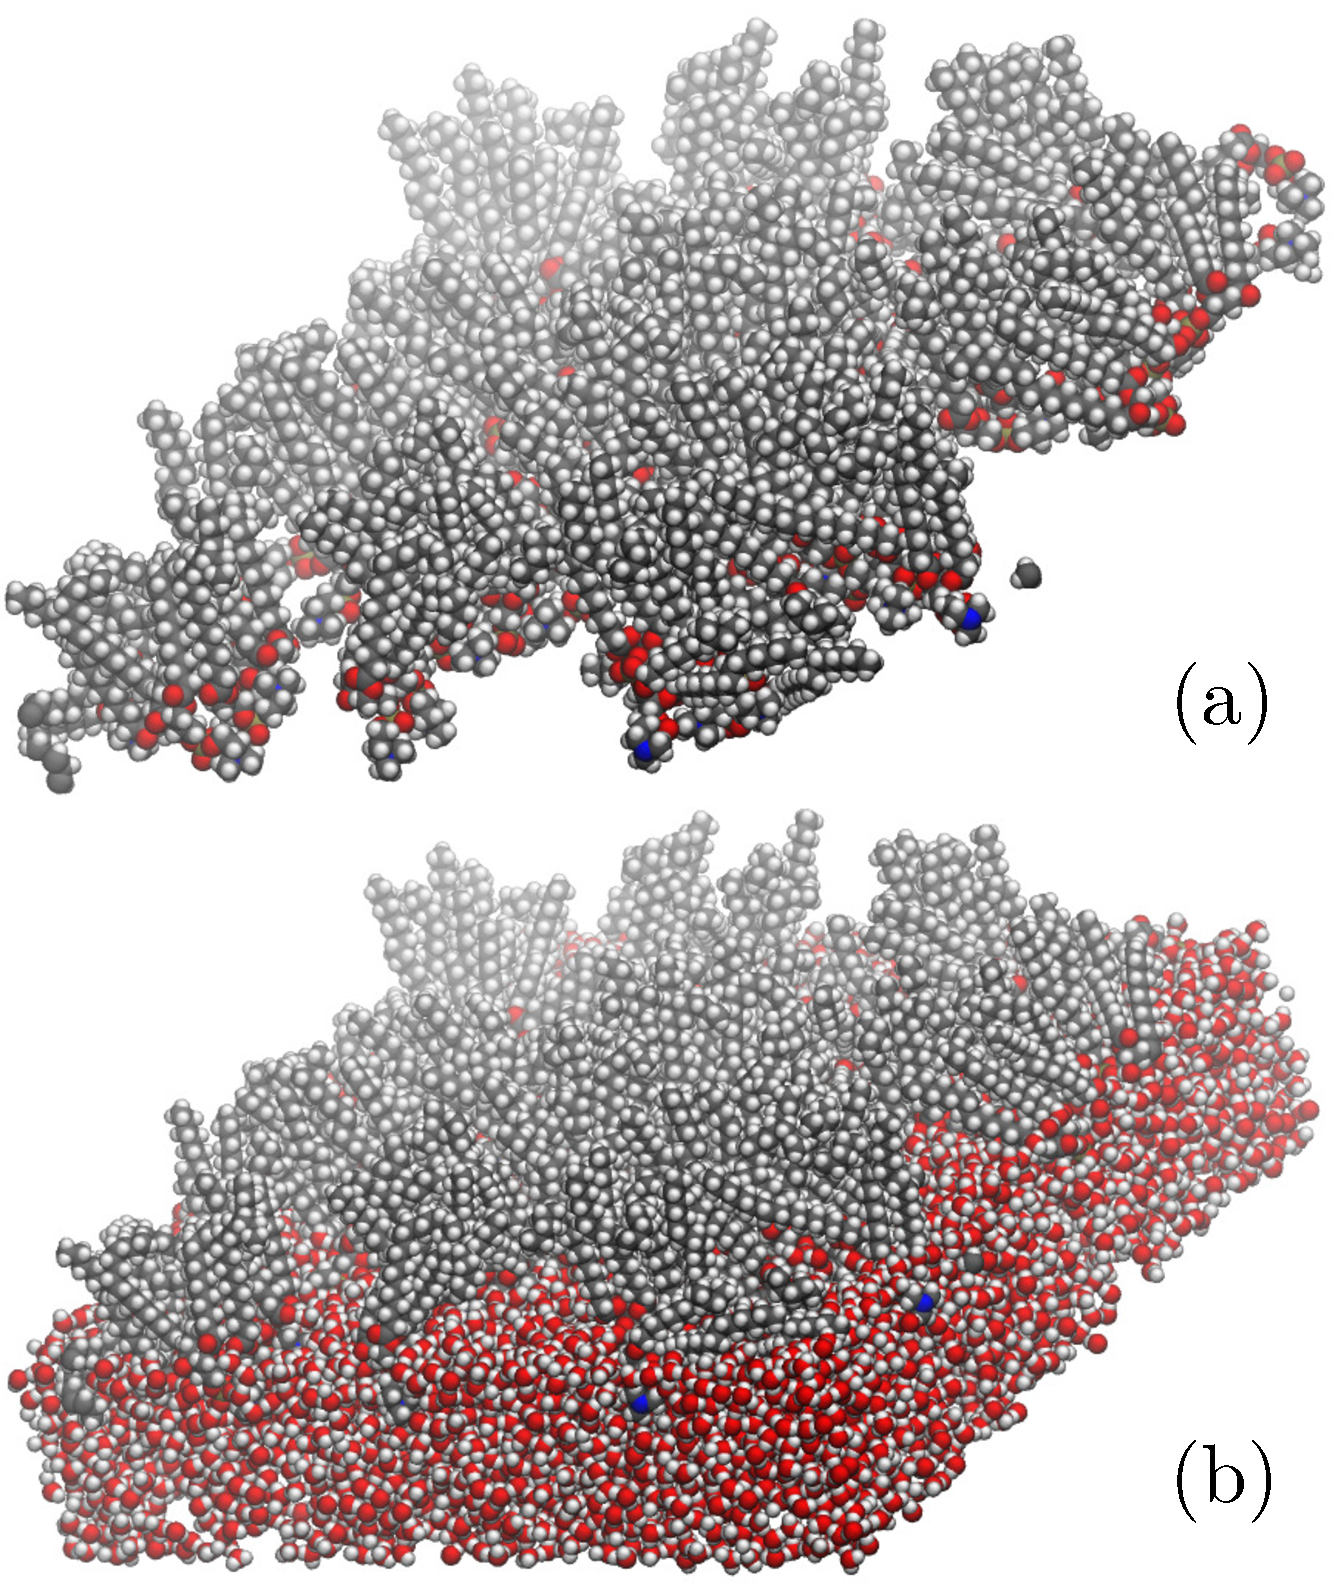
\includegraphics[width=0.60\textwidth]{reflectometry2/dspcdrywet}
    \caption{The DSPC monolayer; (a) without water layer and (b) with water layer, visuallised using VMD (\cite{humphrey_vmd_1996}).}
    \label{fig:drywet}
\end{figure}
%

A general protocol was then used to relax the system at the desired surface coverage, reproducing the effects of a Langmuir trough \emph{in-silico}.
This involved subjecting the system to a semi-isotropic barostat, with compressibility of \SI{4.5e-5}{\per\bar} of the Slipids and Berger simulations and \SI{3.0e-4}{\per\bar} for the MARTINI simulations.
The pressure in the \emph{z}-dimension was kept constant at \SI{1}{\bar}, while it was increased in the \emph{x}- and \emph{y}-dimensions isotropically.
This allowed the surface area of the interface to reduce, as the phospholipid molecules have a preference to stay at the interface, while the total volume of the system stayed relatively constant, as the water molecules move down to relax the pressure in the \emph{z}-dimension.
When the \emph{xy}-area is reached that is associated with the area per molecule\footnote{Abbreviated to APM.} for each SP, described by the experimental SP-isotherm shown in Figure~\ref{fig:surfiso} and given in Table \ref{tab:apm}, the coordinates were saved and used as the starting structure for the equilibration simulation.
This equilibration simulation involved continuing the use of the semi-isotropic barostat, with the \emph{xy}-area of the box fixed, allowing the system to relax at a pressure of \SI{1}{\bar} in the \emph{z}-dimension.
Following the application of the pair of semi-isotropic barostats, the thickness of the water layer was typically in the region of \SI{30}{\angstrom}.
The equilibration period was \SI{1}{\nano\second}, following which the \SI{50}{\nano\second} NVT\footnote{Constant number of particles, volume, and temperature.} ensemble production simulations were run, on which all analyses were conducted.
%
\begin{figure}[t]
    \centering
    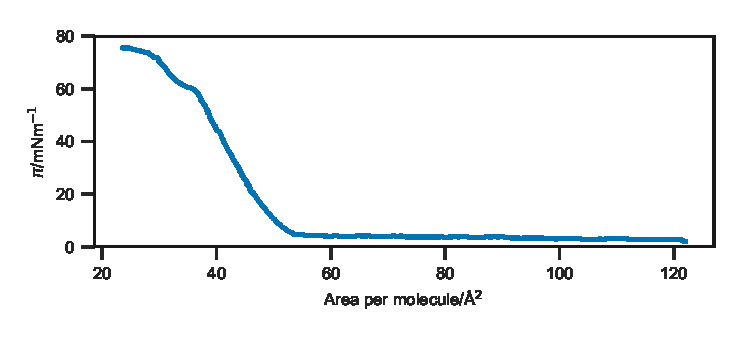
\includegraphics[width=\textwidth]{reflectometry2/apm}
    \caption{The experimental SP-isotherm for DSPC, taken from \cite{kubo_phosphatidylcholine_2001}.}
    \label{fig:surfiso}
\end{figure}
%
%
\begin{table}[b]
    \centering
    \small
    \caption{The areas per molecule (APMs) associated with particular SPs and the size of the \emph{x}- and \emph{y}-cell dimension for a simulation of 100 phospholipid molecules.}
    \label{tab:apm}
    \begin{tabular}{l | l l}
        \toprule
        $\pi$/\si{\milli\newton\per\meter} & APM/\si{\angstrom\squared} & \emph{xy}-cell length/\si{\angstrom} \\
        \midrule
        \num{20} & \num{47.9} & \num{69.1} \\
        \num{30} & \num{46.4} & \num{68.1} \\
        \num{40} & \num{45.0} & \num{67.1} \\
        \num{50} & \num{44.6} & \num{66.0} \\
        \bottomrule
    \end{tabular}
\end{table}
%

\section{Data analysis}
\subsection{Traditional layer-model analysis}
In order to provide a point of comparison for the simulation-derived methods, the chemically-consistent reflectometry model developed in Chapter~\ref{reflectometry1} was used for the analysis of the experimental data.
Two modifications were made to the methodology described in Chapter~\ref{reflectometry1}.
The first was that the volume of the phospholipid tail group, $V_t$ was constrained based on the APM,\footnote{As taken from the surface pressure-isotherm data}
%
\begin{equation}
V_t = d_t\text{APM},
\end{equation}
%
where $d_t$ is the tail layer thickness.
The result of this constraint is that both the monolayer model and the simulation-derived models were constrained equally by the measured surface coverage.
The second modification was to constrain the head group volume to a value of \SI{339.5}{\angstrom}, in agreement with the work of Ku\v{c}erka \emph{et al.}\autocite{kucerka_determination_2004} and Balgav\'{y} \emph{et al.}\autocite{balgavy_evaluation_2001}
This constraint was possible on this occasion as the monolayer was at the air-water interface, compared to the air-DES interface previously.
A uniform background, limited to lie within \SI{10}{\percent} of the highest $q$-vector reflected intensity, and a scale factor were then determined using \texttt{refnx} to offer the best agreement between the calculated reflectometry profile and that measured experimentally.

The experimental data from all seven contrasts were co-refined to a single monolayer model at each surface pressure, where the head thickness, tail thickness, and interfacial roughness were allowed to vary.
The co-refinement of measurements at different surface pressures was not required, as there was a substantial number of contrasts measured.
The values of the head and tail scattering lengths are given in Table~\ref{tab:scat}, while the SLD of the super and subphase were taken as \SI{0}{\per\squared\angstrom}, and \SI{6.35}{\per\squared\angstrom} and \SI{0}{\per\squared\angstrom} respectively.
For each co-refinement of seven neutron reflectometry measurements, there were in total five degrees of freedom in the fitting process, and the fitting was performed using a differential evolution algorithm.
As with the work of Chapter~\ref{reflectometry1}, Markov chain Monte Carlo sampling was used to obtain experimental uncertainties on the fitted model, enabled by the \texttt{emcee} package \cite{foreman-mackey_emcee_2013}.
The same protocol for this sampling was used herein.
%
\begin{table}
\centering
\small
  \caption{The different scattering lengths of the head and tail phospholipid components. }
  \label{tab:scat}
  \begin{tabular}{lllll}
    \toprule
    Contrast & d$_{13}$-DSPC & d$_{70}$-DSPC & d$_{83}$-DSPC & h-DSPC  \\
    \midrule
    $b_{\text{head}}$\SI{10e-4}{\angstrom} & 19.54 & 11.21 & 24.75 & 6.01 \\
    $b_{\text{tail}}$\SI{10e-4}{\angstrom} & -3.58 & 69.32 & 69.32 & -3.58 \\
    \bottomrule
  \end{tabular}
\end{table}
%

\subsection{Simulation-dervied analysis}
A custom-class, \texttt{md\_simulation}, was developed for \texttt{refnx}\autocite{nelson_refnx_2019,nelson_refnx_2019-1} that enabled the determination of a reflectometry profile from simulation, using a similar method to that employed in previous work, such as Dabkowska \emph{et al.}\autocite{dabkowska_modulation_2014}
The Abel\`{e}s layer model formalism is applied to layers, the SLD of which is drawn directly from the simulation, and the thickness of which is defined.
The layer thickness used was \SI{1}{\angstrom} for the Slipid and Berger potential model simulations, with an interfacial roughness between these layers of \SI{0}{\angstrom}.
For the MARTINI potential model, a layer thickness of \SI{4}{\angstrom} was used, with an interfacial roughness of \SI{0.4}{\angstrom}.\footnote{The motivation for this is discussed in Section~\ref{sec:martanal}.}
Each of the \SI{50}{\nano\second} production simulations were analysed each \SI{0.1}{\nano\second}, and the SLD profiles were determined by summing the scattering lengths, $b_j$, for each of the atoms in a given layer.
%
\begin{equation}
\text{SLD}_n = \frac{\sum_j b_j}{V_n},
\end{equation}
%
where, $V_n$ is the volume of the layer $n$, obtained from the simulation cell parameters in the plane of the interface and the defined layer thickness.
A uniform background, limited to lie withing \SI{10}{\percent} of the highest $q$-value reflected intensity, and a scale factor were then determined using \texttt{refnx} to offer the best agreement between the calculated reflectometry profile and that measured experimentally.

\subsection{Comparison between monolayer model and simulation-derived analysis}
In order to assess the agreement between the model from each method, the following goodness-of-fit metric was used, following the transformation of the data into $Rq^4$ space,
%
\begin{equation}
\chi^2 = \sum_{i=1}^{N_{\text{data}}}{\frac{[R_{\text{exp}}(q_i) - R_{\text{sim}}(q_i)]^2}{[\delta R_{\text{exp}}(q_i)]^2}},
\end{equation}
%
where, $q_i$ is a given $q$-vector, $R_{\text{exp}}(q_i)$ is the experimental reflected intensity, $R_{\text{sim}}(q_i)$ is the simulation-derived/traditionally-developed reflected intensity, and $\delta R_{\text{exp}}(q_i)$ is the resolution function of the experimental data.

The number of water molecules per head group\footnote{Abbreviated to wph.} was also compared between the different methods.
This was obtained from the monolayer model by considering the solvent fraction in the head-layer, $\phi_h$, the volume of the head group, $V_h$, and taking the volume of a single water molecule to be \SI{29.9}{\angstrom\cubed},\footnote{Found from the density of water as \SI{997}{\kg\per\meter\cubed}.}
%
\begin{equation}
\text{wph}=\frac{\phi_h V_h}{29.9 - 29.9\phi_h}.
\label{equ:wph}
\end{equation}
%
In MD simulations, the number densities, in the \emph{z}-dimension, for each of the three components\footnote{The phospholipid heads, phospholipid tails, and water.} may be obtained directly from the trajectory.
In order to determine the number of water molecules per headgroup from the MD simulations, a head-layer region was defined of that which contained the middle \SI{60}{\percent} of the phospholipid head number density.
The ratio between the water density and the phospholipid head density was then found within thei head-layer region.

\subsection{Simulation trajectory analysis}
\label{sec:traj}
In order to use the MD trajectory to guide the future development of the chemically-consistent layer model, it was necessary to investigate the solvent penetration into the head group regions of the phospholipids, the roughness of each interface and the phospholipid tail length.
The solvent penetration was determined using the intrinsic surfact approach, as deatiled by Allen \emph{et al.}\autocite{allen_specific_2016,pandit_algorithm_2003}
The intrinsic surface approach enables the calculation of the solvent penetration without the effect of the monolayer roughness.
This involves taking the \emph{z}-dimension position of each atom with respect to an anchor point, in this work the anchor point was taken as the phosphorus atom of the phospholipid head that was closest to the atom in the \emph{xy}-plane.
The roughness was probed by investigating the variation in positions from the start, middle and end of each of the head and tail groups.
The start of the phospholipid head was defined as the nitrogen atom, the middle the phosphorus and the end the tertiary carbon, which the start of the phospholipid tail was defined as the carbonyl carbon atom, the middle the ninth carbon in the tail, and the end the final carbon in the tail.
The distribution of each of these atom types was determined by finding the \SI{95}{\percent} quantile for the position in the \emph{z}-dimension and comparing the spread of the mean and the upper quantile.
Finally, the tail length distance, $t_t$, was found as the distance from the carbonyl carbon atom to the final primary carbon atom of the phospholipid tail.
All of these analyses used the \texttt{MDAnalysis} package.\autocite{gowers_mdanalysis_2016,michaud-agrawal_mdanalysis_2011}

\section{Results \& Discussion}
Figures~\ref{fig:dspcccref} to \ref{fig:dspcmartref} compare the reflectometry and SLD profiles from each of the different methods at each surface pressure.
It is clear that the trends for all surface pressures are similar.
In addition, the $\chi^2$ between each of the models and the experimental data for each contrast at an APM associated with a surface pressure of \SI{30}{\milli\newton\per\meter}, the average $\chi^2$ and standard deviation for each method are given in Table~\ref{tab:chi}.
%
\begin{figure}
    \centering
    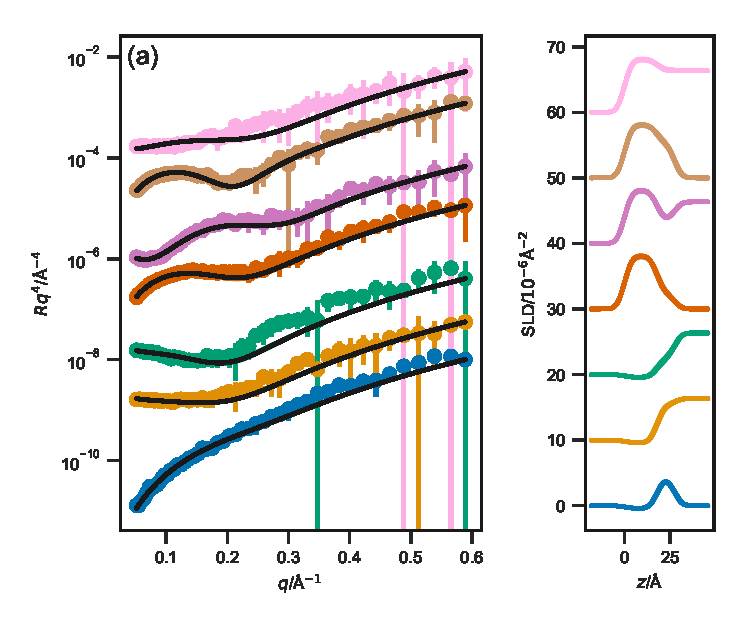
\includegraphics[width=0.49\textwidth]{reflectometry2/dspc_20_ref_sld}
    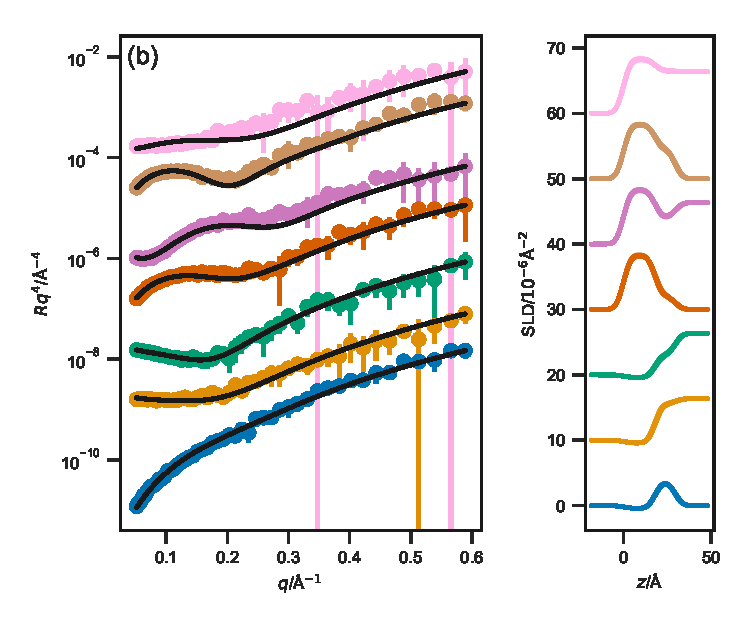
\includegraphics[width=0.49\textwidth]{reflectometry2/dspc_30_ref_sld}\\
    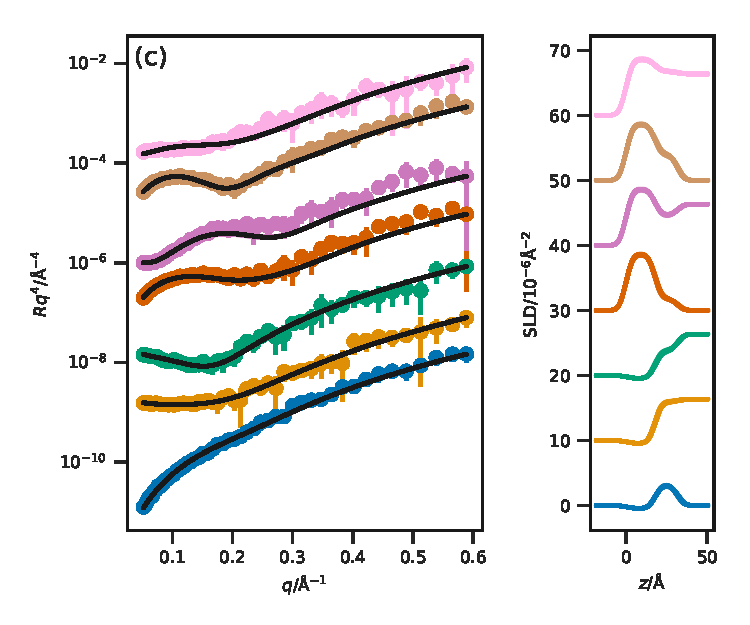
\includegraphics[width=0.49\textwidth]{reflectometry2/dspc_40_ref_sld}
    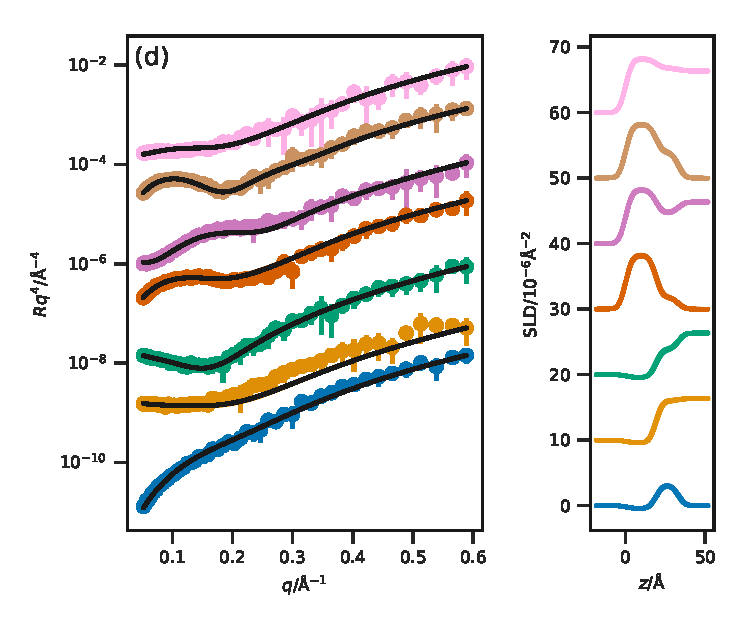
\includegraphics[width=0.49\textwidth]{reflectometry2/dspc_50_ref_sld}
    \caption{The NR profiles (left) and SLD profiles (right) determined from the chemically-consistent model for DSPC; (a) at \SI{20}{\milli\newton\per\meter}, (b) at \SI{30}{\milli\newton\per\meter}, (c) at \SI{40}{\milli\newton\per\meter}, and (d) at \SI{50}{\milli\newton\per\meter}. From top-to-bottom the contrasts are as follows; d${_83}$-\ce{D2O}, d${_83}$-ACMW, d${_70}$-\ce{D2O}, d${_70}$-ACMW, h-\ce{D2O}, d${_13}$-\ce{D2O}, d${_13}$-ACMW. The different contrast NR profiles have been offset in the \emph{y}-axis by an order of magnitude and the SLD profiles offset in the \emph{y}-axis by \SI{10e-6}{\per\angstrom\squared}, for clarity.}
    \label{fig:dspcccref}
\end{figure}
%
%
\begin{figure}
    \centering
    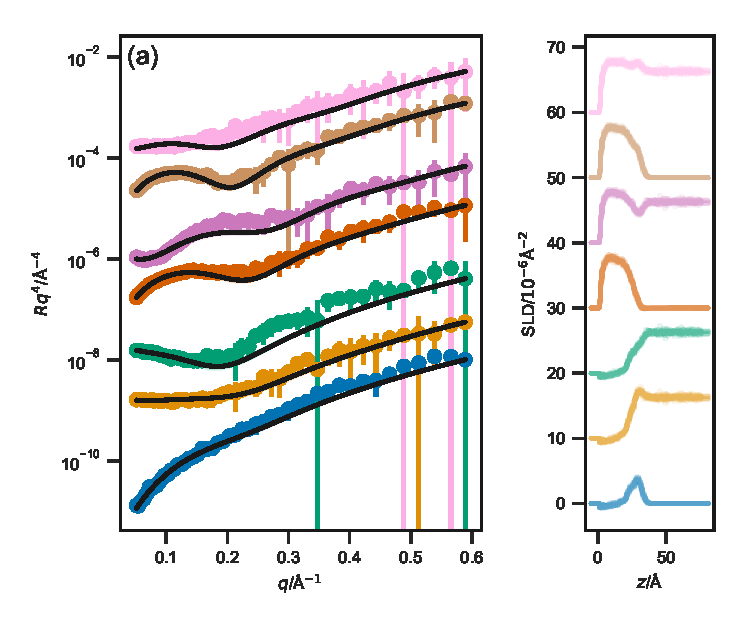
\includegraphics[width=0.49\textwidth]{reflectometry2/dspc_slipids_20_ref_sld}
    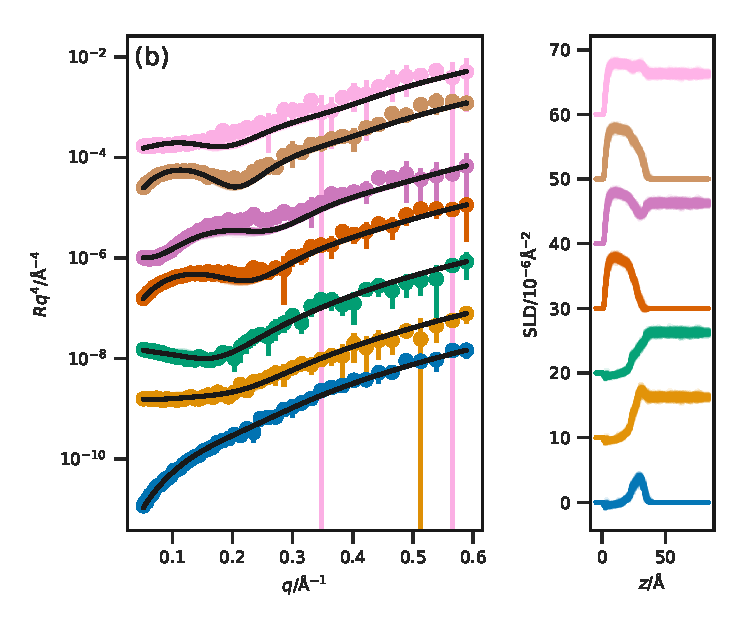
\includegraphics[width=0.49\textwidth]{reflectometry2/dspc_slipids_30_ref_sld}\\
    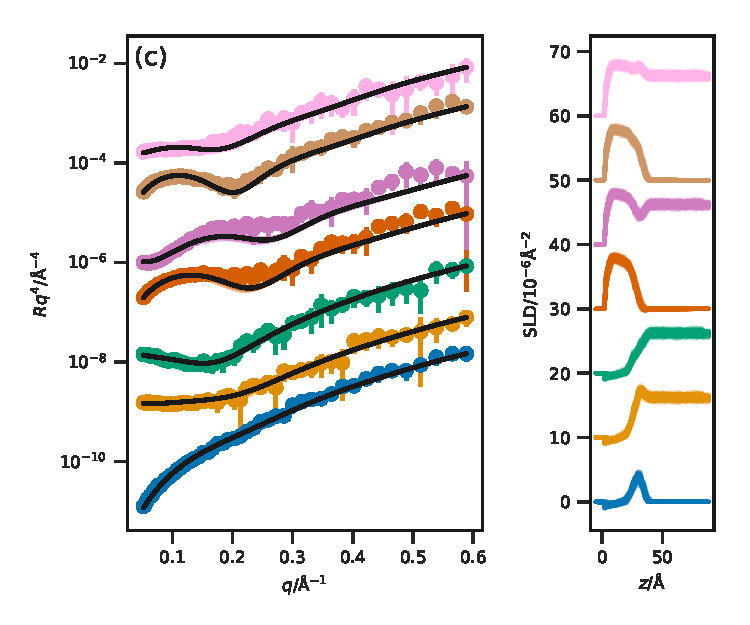
\includegraphics[width=0.49\textwidth]{reflectometry2/dspc_slipids_40_ref_sld}
    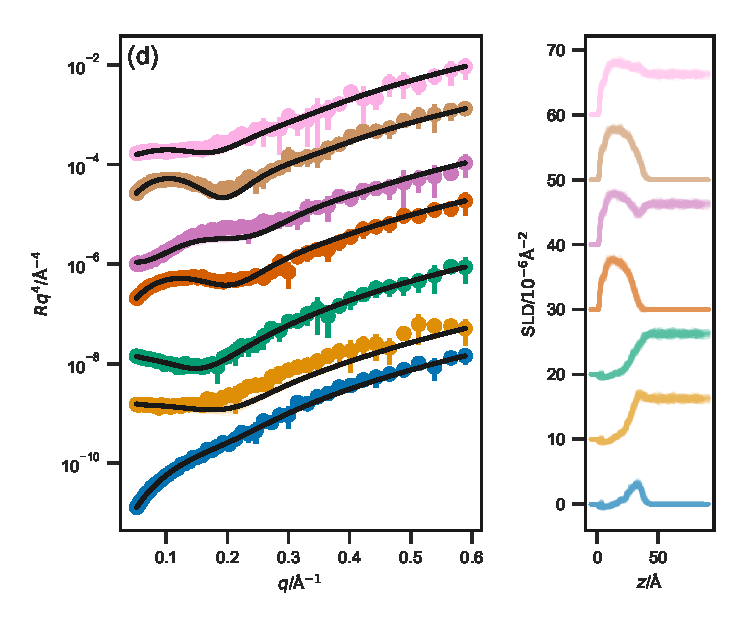
\includegraphics[width=0.49\textwidth]{reflectometry2/dspc_slipids_50_ref_sld}
    \caption{The NR profiles (left) and SLD profiles (right) determined from the Slipid all-atom potential model simulations of DSPC; (a) at \SI{20}{\milli\newton\per\meter}, (b) at \SI{30}{\milli\newton\per\meter}, (c) at \SI{40}{\milli\newton\per\meter}, and (d) at \SI{50}{\milli\newton\per\meter}. From top-to-bottom the contrasts are as follows; d${_83}$-\ce{D2O}, d${_83}$-ACMW, d${_70}$-\ce{D2O}, d${_70}$-ACMW, h-\ce{D2O}, d${_13}$-\ce{D2O}, d${_13}$-ACMW. The different contrast NR profiles have been offset in the \emph{y}-axis by an order of magnitude and the SLD profiles offset in the \emph{y}-axis by \SI{10e-6}{\per\angstrom\squared}, for clarity.}
    \label{fig:dspcsliref}
\end{figure}
%
%
\begin{figure}
    \centering
    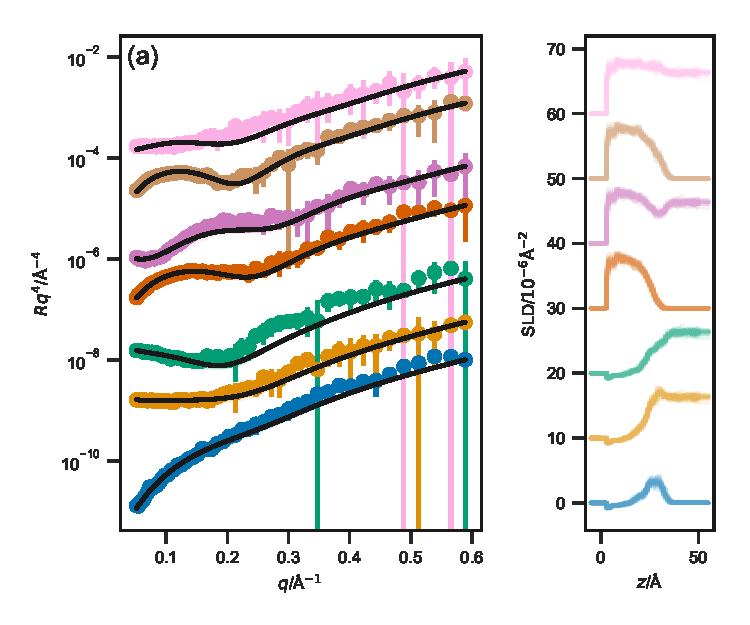
\includegraphics[width=0.49\textwidth]{reflectometry2/dspc_berger_20_ref_sld}
    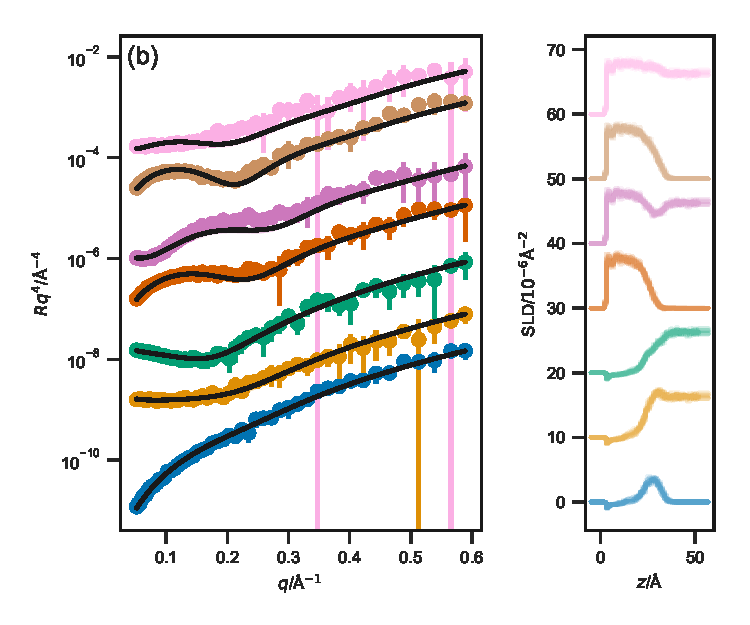
\includegraphics[width=0.49\textwidth]{reflectometry2/dspc_berger_30_ref_sld}\\
    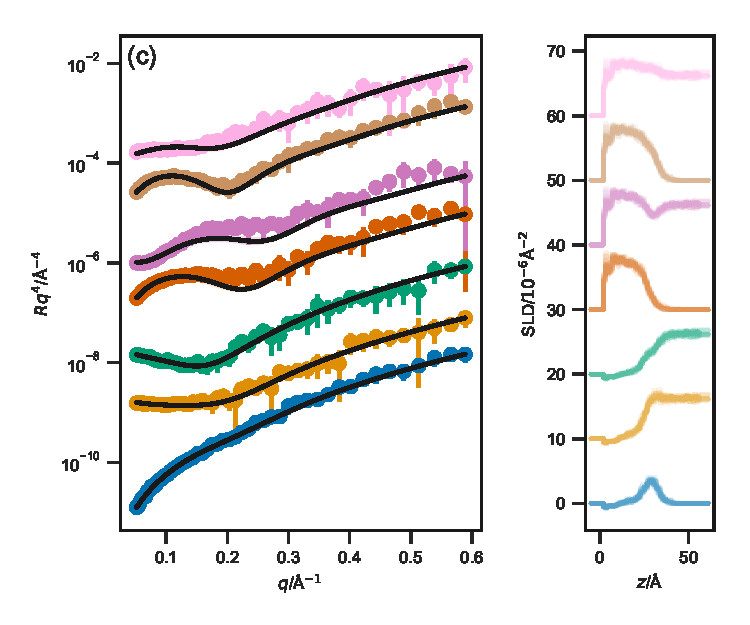
\includegraphics[width=0.49\textwidth]{reflectometry2/dspc_berger_40_ref_sld}
    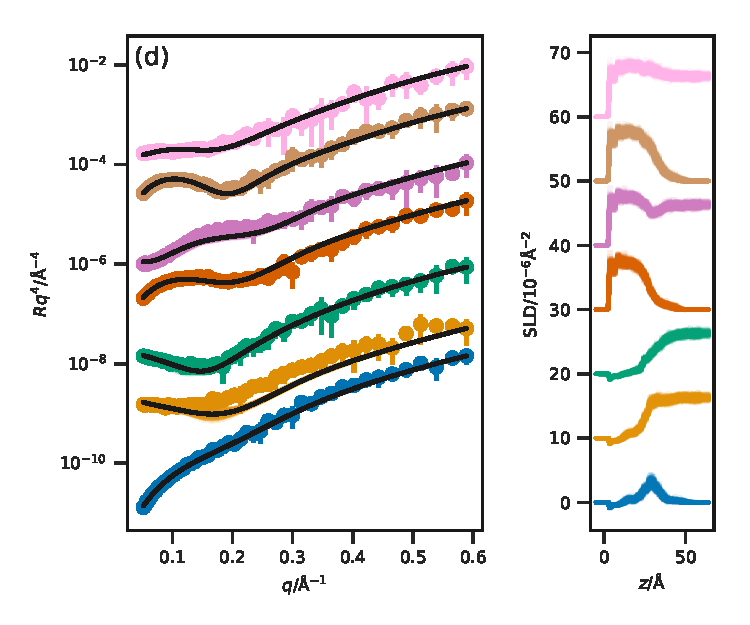
\includegraphics[width=0.49\textwidth]{reflectometry2/dspc_berger_50_ref_sld}
    \caption{The NR profiles (left) and SLD profiles (right) determined from the Berger united-atom potential model simulations of DSPC; (a) at \SI{20}{\milli\newton\per\meter}, (b) at \SI{30}{\milli\newton\per\meter}, (c) at \SI{40}{\milli\newton\per\meter}, and (d) at \SI{50}{\milli\newton\per\meter}. From top-to-bottom the contrasts are as follows; d${_83}$-\ce{D2O}, d${_83}$-ACMW, d${_70}$-\ce{D2O}, d${_70}$-ACMW, h-\ce{D2O}, d${_13}$-\ce{D2O}, d${_13}$-ACMW. The different contrast NR profiles have been offset in the \emph{y}-axis by an order of magnitude and the SLD profiles offset in the \emph{y}-axis by \SI{10e-6}{\per\angstrom\squared}, for clarity.}
    \label{fig:dspcberref}
\end{figure}
%
%
\begin{figure}
    \centering
    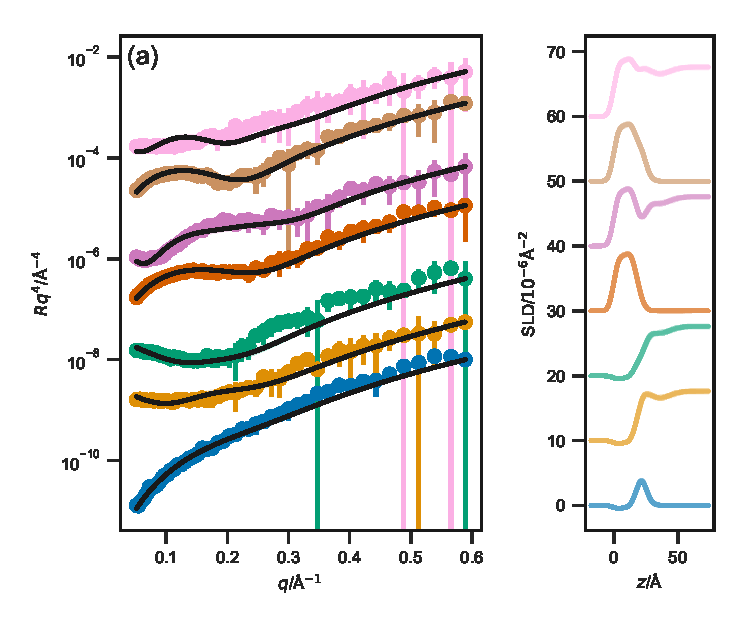
\includegraphics[width=0.49\textwidth]{reflectometry2/dspc_martini_20_ref_sld}
    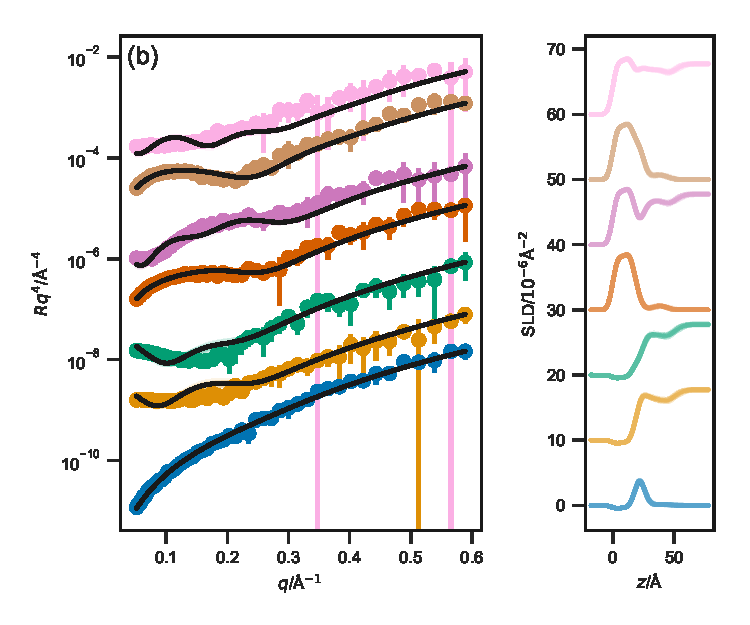
\includegraphics[width=0.49\textwidth]{reflectometry2/dspc_martini_30_ref_sld}\\
    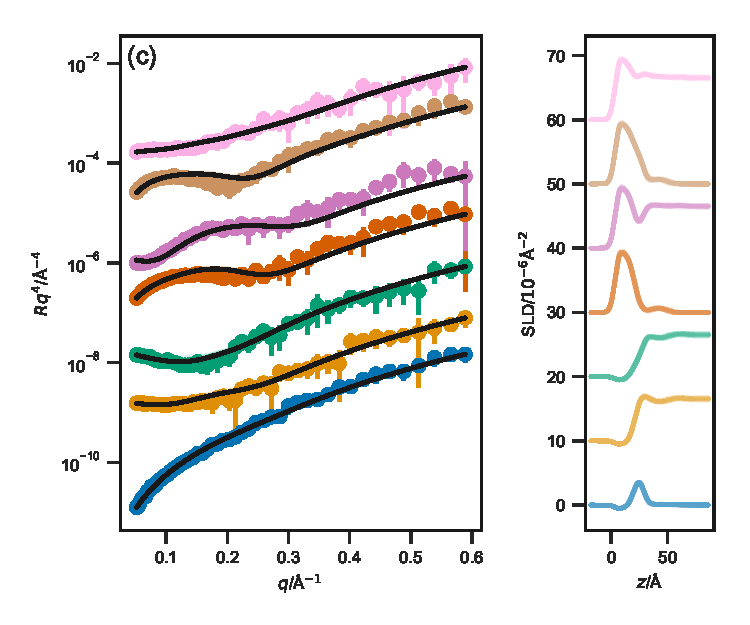
\includegraphics[width=0.49\textwidth]{reflectometry2/dspc_martini_40_ref_sld}
    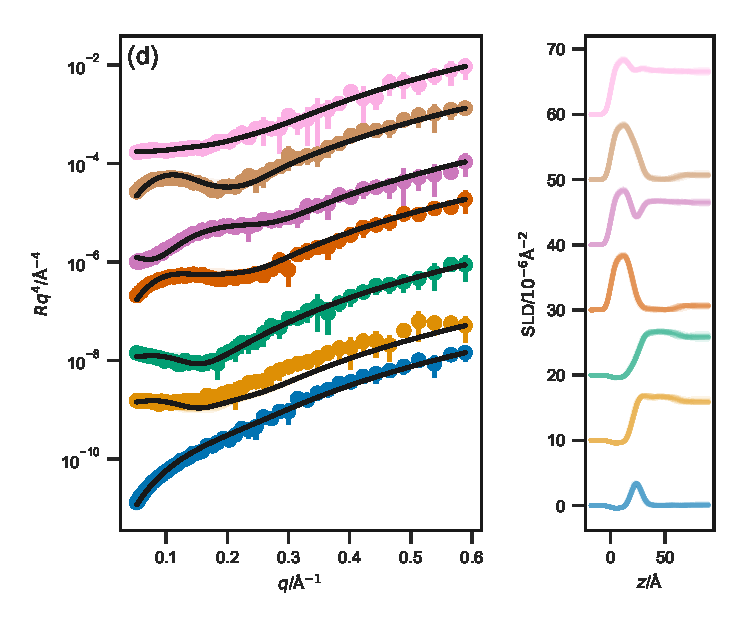
\includegraphics[width=0.49\textwidth]{reflectometry2/dspc_martini_50_ref_sld}
    \caption{The NR profiles (left) and SLD profiles (right) determined from the MARTINI coarse-grained potential model simulations of DSPC; (a) at \SI{20}{\milli\newton\per\meter}, (b) at \SI{30}{\milli\newton\per\meter}, (c) at \SI{40}{\milli\newton\per\meter}, and (d) at \SI{50}{\milli\newton\per\meter}. From top-to-bottom the contrasts are as follows; d${_83}$-\ce{D2O}, d${_83}$-ACMW, d${_70}$-\ce{D2O}, d${_70}$-ACMW, h-\ce{D2O}, d${_13}$-\ce{D2O}, d${_13}$-ACMW. The different contrast NR profiles have been offset in the \emph{y}-axis by an order of magnitude and the SLD profiles offset in the \emph{y}-axis by \SI{10e-6}{\per\angstrom\squared}, for clarity.}
    \label{fig:dspcmartref}
\end{figure}
%
%
\begin{table}
    \centering
    \small
    \caption{The $\chi^2$ values for each of the reflectometry models at an APM associated with a surface pressure of \SI{30}{\milli\newton\per\meter}.}
    \label{tab:chi}
    \begin{tabular}{l | l l l l}
        \toprule
        Contrast & Chemically-consistent & Slipids & Berger & MARTINI \\
        \midrule
        h-\ce{D2O} & \input{output/reflectometry2/dspc_30/dspc_30_hd2o_chi.txt} & \input{output/reflectometry2/dspc_30/dspc_slipids_30_hd2o_chi.txt} & \input{output/reflectometry2/dspc_30/dspc_berger_30_hd2o_chi.txt} & \input{output/reflectometry2/dspc_30/dspc_martini_30_hd2o_chi.txt} \\
        d$_{13}$-\ce{D2O} & \input{output/reflectometry2/dspc_30/dspc_30_d13d2o_chi.txt} & \input{output/reflectometry2/dspc_30/dspc_slipids_30_d13d2o_chi.txt} & \input{output/reflectometry2/dspc_30/dspc_berger_30_d13d2o_chi.txt} & \input{output/reflectometry2/dspc_30/dspc_martini_30_d13d2o_chi.txt} \\
        d$_{13}$-ACMW & \input{output/reflectometry2/dspc_30/dspc_30_d13acmw_chi.txt} & \input{output/reflectometry2/dspc_30/dspc_slipids_30_d13acmw_chi.txt} & \input{output/reflectometry2/dspc_30/dspc_berger_30_d13acmw_chi.txt} & \input{output/reflectometry2/dspc_30/dspc_martini_30_d13acmw_chi.txt} \\
        d$_{70}$-\ce{D2O} & \input{output/reflectometry2/dspc_30/dspc_30_d70d2o_chi.txt} & \input{output/reflectometry2/dspc_30/dspc_slipids_30_d70d2o_chi.txt} & \input{output/reflectometry2/dspc_30/dspc_berger_30_d70d2o_chi.txt} & \input{output/reflectometry2/dspc_30/dspc_martini_30_d70d2o_chi.txt} \\
        d$_{70}$-ACMW & \input{output/reflectometry2/dspc_30/dspc_30_d70acmw_chi.txt} & \input{output/reflectometry2/dspc_30/dspc_slipids_30_d70acmw_chi.txt} & \input{output/reflectometry2/dspc_30/dspc_berger_30_d70acmw_chi.txt} & \input{output/reflectometry2/dspc_30/dspc_martini_30_d70acmw_chi.txt} \\
        d$_{83}$-\ce{D2O} & \input{output/reflectometry2/dspc_30/dspc_30_d83d2o_chi.txt} & \input{output/reflectometry2/dspc_30/dspc_slipids_30_d83d2o_chi.txt} & \input{output/reflectometry2/dspc_30/dspc_berger_30_d83d2o_chi.txt} & \input{output/reflectometry2/dspc_30/dspc_martini_30_d83d2o_chi.txt} \\
        d$_{83}$-ACMW & \input{output/reflectometry2/dspc_30/dspc_30_d83acmw_chi.txt} & \input{output/reflectometry2/dspc_30/dspc_slipids_30_d83acmw_chi.txt} & \input{output/reflectometry2/dspc_30/dspc_berger_30_d83acmw_chi.txt} & \input{output/reflectometry2/dspc_30/dspc_martini_30_d83acmw_chi.txt} \\
        \midrule
        Average & \input{output/reflectometry2/dspc_30/dspc_30_all_chi.txt} & \input{output/reflectometry2/dspc_30/dspc_slipids_30_all_chi.txt} & \input{output/reflectometry2/dspc_30/dspc_berger_30_all_chi.txt} & \input{output/reflectometry2/dspc_30/dspc_martini_30_all_chi.txt} \\
        \bottomrule
    \end{tabular}
\end{table}
%

\subsection{Traditional analysis}
The chemically-consistent model was used to determine the structure of the lipid monolayer, Table~\ref{tab:cc} gives the optimum values for the parameters that were varied in the model.
It is clear from this Table, that as the surface pressure is increased, as expected (and as found previously \cite{mohwald_phospholipid_1990,vaknin_structural_1991}), the overall thickness of the monolayer increases.
The thickness increase for the lipid tails may be associated with the straightening of the tails with respect to the interface normal, while the thickness increase of the head groups has been noted previously for DSPC \cite{hollinshead_effects_2009}.
%
\begin{table*}
\small
  \caption{\ The values for the parameters allowed to vary in the fitting of the chemically-consistent model, at each surface pressure measured.}
  \label{tab:cc}
  \begin{tabular*}{\textwidth}{@{\extracolsep{\fill}}llllll}
    \hline
    Surface Pressure/\si{\milli\newton\per\meter} & $d_h$/\si{\angstrom} & $d_t$/\si{\angstrom} & $\sigma_{t,h,s}$/\si{\angstrom} & $\phi_h$$\times10^{-2}$ & $V_t$/\si{\angstrom\cubed} \\
    \hline
    20 & \input{output/reflectometry2/dspc_20/dspc_20-d_h_20.tex} & \input{output/reflectometry2/dspc_20/dspc_20-d_t_20.tex} & \input{output/reflectometry2/dspc_20/dspc_20_rough_20.tex} & \input{output/reflectometry2/dspc_20/dspc_20-phih_20.tex} & \input{output/reflectometry2/dspc_20/dspc_20-V_t_20.tex} \\
    30 & \input{output/reflectometry2/dspc_30/dspc_30-d_h_30.tex} & \input{output/reflectometry2/dspc_30/dspc_30-d_t_30.tex} & \input{output/reflectometry2/dspc_30/dspc_30_rough_30.tex} & \input{output/reflectometry2/dspc_30/dspc_30-phih_30.tex} & \input{output/reflectometry2/dspc_30/dspc_30-V_t_30.tex} \\
    40 & \input{output/reflectometry2/dspc_40/dspc_40-d_h_40.tex} & \input{output/reflectometry2/dspc_40/dspc_40-d_t_40.tex} & \input{output/reflectometry2/dspc_40/dspc_40_rough_40.tex} & \input{output/reflectometry2/dspc_40/dspc_40-phih_40.tex} & \input{output/reflectometry2/dspc_40/dspc_40-V_t_40.tex} \\
    50 & \input{output/reflectometry2/dspc_50/dspc_50-d_h_50.tex} & \input{output/reflectometry2/dspc_50/dspc_50-d_t_50.tex} & \input{output/reflectometry2/dspc_50/dspc_50_rough_50.tex} & \input{output/reflectometry2/dspc_50/dspc_50-phih_50.tex} & \input{output/reflectometry2/dspc_50/dspc_50-V_t_50.tex} \\
    \hline
  \end{tabular*}
\end{table*}
%

It would be anticipated that as the surface pressure increases, there would be a corresponding decrease in the volume fraction of solvent in the head group \cite{bayerl_specular_1990}.
However, for DSPC, the volume fraction of the solvent appears to be constant (or even increase slightly) with increasing surface pressure.
We believe that this is due to the decision to constrain the volume of the lipid head, which may decrease with increasing surface pressure.
It has been noted previously that the interfacial roughness will increase with increasing surface pressure \cite{lu_aspects_1994}, this can be observed with the slight increase between \SIrange{20}{50}{\milli\newton\per\meter}.

Hollinshead \emph{et al.} \cite{hollinshead_effects_2009} suggest a tail volume of \SI{972}{\angstrom\cubed} from the density data.
However, the values found in this work are substantially lower, at \SI{\sim850}{\angstrom\cubed}.
This reduction, of \SI{\sim12}{\percent}, agrees well with the work of Campbell \emph{et al.} \cite{campbell_structure_2018} and Small \cite{small_lateral_1984}, which suggest that under the surface pressure investigated in this work a reduction of the tail volume of up to \SI{15}{\percent} may be observed.
We believe that the model layer structure from the chemically-consistent method provides a satisfactory description of the monolayer structure.
However, the use of an MD-driven analysis method may provide greater insight into the chemical nature of the monolayer.

\subsection{MARTINI}
Initially, the MARTINI coarse-grained simulations were analysed with a layer thickness of \SI{1}{\angstrom} and an interfacial roughness of \SI{0}{\angstrom}, in a similar fashion to the other potential models.
However, as can be seen in Figure~\ref{fig:martorder} there is a clear ordering effect present in the MARTINI water, despite the use of the polarised water model.
The effect of this ordering on the SLD profile, and therefore the reflectometry profile, can be reduced by using a larger layer thickness and introducing an interfacial roughness.
Therefore, in the results discussed below the MARTINI potential model simulation were analysed using a layer thickness of \SI{4}{\angstrom} and an interfacial roughness of \SI{0.4}{\angstrom}.
It is noted that this structuring may be reduced through the use of a less ordered wall \cite{koutsioubas_combined_2016} at the extreme of the simulation cell, however, the aim was to reproduce the experimental conditions using off-the-shelf tools and this would require custom modifications not easily available.
Alternatively, it may be possible to effect the presence of this structuring through the inclusion of \SI{\sim 10}{\percent} of antifreeze MARTINI beads alongside the normal MATRINI water.
However, this method has been noted to also give structuring effects in the presence on an ordered wall \cite{marrink_comment_2010}.
%
\begin{figure}
    \centering
    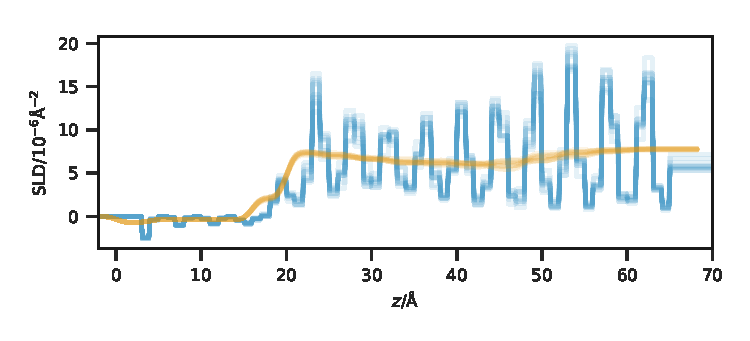
\includegraphics[width=0.80\textwidth]{reflectometry2/martini_order}
    \caption{A comparison of the scattering length density profile for the MARTINI potential model simulations at an APM associated with a surface pressure of \SI{30}{\milli\newton\per\meter}; the blue line shows the data where the layer thickness was \SI{1}{\angstrom} and no interfacial roughness and the orange line shows that with a layer thickness of \SI{4}{\angstrom} and a roughness of \SI{0.4}{\angstrom}}
    \label{fig:martorder}
\end{figure}
%

It can be seen from Table~\ref{tab:chi} and Figure~\ref{fig:dspcmartref} that even with the larger layer thickness and adding interlayer roughness, the MARTINI potential model simulations do not effectively reproduce the reflectometry profile.
Furthermore, it is noted that the agreement with the contrasts containing \ce{D2O} is particularly poor.
This is most likely an artefact of the structuring effect mentioned above which cannot be completely removed.

However, the agreement for the samples where the contrast uses ACMW, where the water is effectively removed from the SLD profile is also poor.
This indicates that there are other artefacts limiting the applicability of the MARTINI potential model.
Another such artefact is clear from investigating the calculated length of the hydrocarbon tail from the MARTINI simulation, at an APM associated with a surface pressure of \SI{30}{\milli\newton\per\meter}, which was found to be \input{output/reflectometry2/dspc_30/dspc_martini_30_dt.txt}~\si{\angstrom}, significantly less than the \SI{24.3}{\angstrom} estimated by the Tanford equation \cite{tanford_hydrophobic_1980}.
This is due to the nature of the MARTINI's 4-to-1 beading process, as DSPC has a hydrocarbon tail consisting of 18 carbon atoms, and it is not possible to bead such a chain accurately with the MARTINI potential model.
In this work, a MARTINI phospholipid molecule was used with 4 MARTINI beads making up the chain; corresponding to an all-atom hydrocarbon chain of 16 atoms.
Applying the Tanford equation to a hydrocarbon chain of such a length results in an anticipated length of \SI{18.7}{\angstrom}, which agrees better with that found from the simulation.

In addition to the disagreement from the tail beading process, there is also a clear problem with respect to the solvation of the head layer by polarisable water beads.
It can be seen that the number of water molecules per head group in the MARTINI potential model is typically \input{output/reflectometry2/dspc_30/dspc_martini_30_wph.txt}, this is the value at an APM associated with a surface pressure of \SI{30}{\milli\newton\per\meter}.
The chemically-consistent model, however, gives a value of \input{output/reflectometry2/dspc_30/dspc_30-wph_30.tex}.
It is clear that the 4-to-1 beading present in the MARTINI potential model is creating water molecules that are too large to intercalate into the head layer structure, causing a reduction in the number of waters per head group.

The requirement for a 4-to-1 beading strategy for the MARTINI potential model is a significant weakness.
A better method may be limiting experiments to a system that can be modelled exactly or the use of a different beading model.
However, we are not aware of an off-the-shelf coarse-grained potential model that would easily offer the exact beading of DSPC.

\subsection{Comparison with other simulations}
Table~\ref{tab:chi} shows that both the Slipid and Berger potential model simulations agree well with the experimental data, with the Slipid potential model offering a slight improvement over the Berger.
The quality of agreement between these higher-resolution potential models and the chemically-consistent model is relatively similar.
However, the chemically-consistent model still offers a better fit to the experimental data than those determined from DM simulation.

The result that the chemically-consistent model offers better agreement with the data than those from even all-atom simulations is to be expected.
However, simply by considering the level of constraint present implicity when determining the reflectometry profile directly from the simulation.
While the chemically-consistent model constrains the layer model to ensure that the number of phospholipid head groups is the same as the pairs of tail groups, those from MD simulation have more realistic chemical constraints present from the potential model; e.g. bonding of atoms, and the non-bonded potentials.
The quality of the agreement from this multi-modal approach is sufficient for such a method to be applied regularly to the analysis of neutron reflectometry.

Both the Slipid and Berger potential model simulations produced values for the tail length that were in better agreement with that from the Tanford equation than the MARTINI potential model simulations.
For the Slipid potential model, with simulations at an APM associated with a surface pressure of \SI{30}{\milli\newton\per\meter} the tail length was found to be \input{output/reflectometry2/dspc_30/dspc_slipids_30_dt.txt}~\si{\angstrom}, while for the Berger potential model, at the same APM, a value of \input{output/reflectometry2/dspc_30/dspc_berger_30_dt.txt}~\si{\angstrom} was obtained.
Neither is quite as large as the \SI{24.3}{\angstrom} from the Tanford equation, however, it should be noted that this value is considered a theoretical maximum for a fully extended carbon chain, which is unlikely to occur, in a liquid phase monolayer, in reality due to entropic considerations

Using the molecular dynamics simulations and the chemically-consistent model, it is possible to compare the number of water molecules per head group.
From the Slipid and Berger potential model simulations, the number of water molecules per head group at an APM associated with a surface pressure of \SI{30}{\milli\newton\per\meter} was found to be \input{output/reflectometry2/dspc_30/dspc_slipids_30_wph.txt} and \input{output/reflectometry2/dspc_30/dspc_berger_30_wph.txt} respectively.
These are in good agreement with the value of \input{output/reflectometry2/dspc_30/dspc_30-wph_30.tex} found from the chemically-consistent model, using Equation~\ref{equ:wph}.

It should be noted that to obtain the \SI{50}{\nano\second} production run simulation using the all-atom Slipid potential model required over 13 days of using 32 cores of the SCARF computing resource.
This is non-trivial and therefore not necessarily applicable to all neutron reflectometry measurements.
However, the use of a \SI{2}{\femto\second} timestep coudl reduce this time significantly.
Additionally, Figure \ref{fig:short} shows the results from the first \SI{5}{\nano\second} of the Slipid potential model simulations, at an APM assocated with a surface pressure of \SI{30}{\milli\newton\per\meter}, and already good agreement with the data is apparent.
It is important to acknowledge that the length of simulation required may be extremely system specific.
Furthermore, recent developments of molecular dynamics simulations of graphical processing units (GPUs) may allow for significant speed up of the simulations.
The nearly as accurate Berger potential model simulations (which are only marginally less accurate), only approximately 2 days of the same compute resource was required.
This suggests that by using the a larger timestep, shorter simulations, and the power of GPU-based molecular dynamics engines, it may be possible to run these simulations alongside experiments at large facilities to aid interpretation and analysis.
%
\begin{figure}
    \centering
    \includegraphics[width=0.85\textwidth]{reflectometry2/dspc_slipids_30_ref_sld_short}
    \caption{The reflectometry and SLD profiles obtained from the first \SI{5}{\nano\second} of the Slipid potential model simulation, at an APM associated with a surface pressure of \SI{30}{\milli\newton\per\meter}. From top-to-bottom the contrasts are as follows; \ce{d_{83}}-\ce{D2O}, \ce{d_{83}}-ACMW, \ce{d_{70}}-\ce{D2O}, \ce{d_{70}}-ACMW, h-\ce{D2O}, \ce{d_{13}}-\ce{D2O}, \ce{d_{13}}-ACMW. The different contrast reflectometry profiles have been offset in the \emph{y}-axis by an order of magnitude and the SLD profiles offset in the \emph{y}-axis by \SI{10e-6}{\per\square\angstrom}, for clarity.}
    \label{fig:short}
\end{figure}
%

\subsection{Using the Slipid potential model simulations to improve the monolayer model}
Despite the chemically-consistent model offering a small improvement in agreement over the Slipid potential model simulation, we believe that it is possible to use the MD simulations to improve the existing this model.
A possible improvement can be found from considering Figure~\ref{fig:waters}, which shows the solvent penetration of the lipid heads, using the intrinsic surface approach to remove the effect of the interfacial roughness.
It is clear that the plot is not step-wise as is obtained from the uniform solvation model that is commonly used in traditional layer models.
Nor is the distribution sigmoidal, as there is a small deviation in the region of the ester group of the lipid heads.
This is either due ot the hydrophilic interaction of the carbonyl moiety or from pockets of water forming at the air-water interface.
Regardless of the mechanism, this suggests that a different solvation model should be considered for a realistic description of the solvent penetration.
%
\begin{figure}
    \centering
    \includegraphics[width=0.85\textwidth]{reflectometry2/water_20}
    \includegraphics[width=0.85\textwidth]{reflectometry2/water_30}
    \includegraphics[width=0.85\textwidth]{reflectometry2/water_40}
    \includegraphics[width=0.85\textwidth]{reflectometry2/water_50}
    \caption{The simulation time-averaged intrinsic density profile of the water molecules (blue dots), and lipid components (head groups: green dots, tail groups: red dots), where the phosphorus atoms of the lipid heads create the intrinsic surface at $z=0$\si{\angstrom}, and the equivalent number density from the chemically-consistent model (orange line).}
    \label{fig:waters}
\end{figure}
%

Figure~\ref{fig:waters} also shows that without the presense of the roughness, the distribution of the head groups is relatively normal.
This agrees well with the model used previously to fit the experimental data by Hollinshead \emph{et al.} \cite{hollinshead_effects_2009}, where Gaussian functions where used to describe the lipid head and tail groups.
However, the tail group distribution is not Gaussian and this previous method failed to include any additional factors to account for interfacial roughness.
Previous work has suggested that when only a single lipid type is present, the roughness between the layers should be conformal in nature, that is it should be carried uniformly through the layers \cite{kozhevnikov_general_2012,campbell_structure_2018}.
However, from the investigation of the SLD profiles in Figure~\ref{fig:dspcsliref} it appears that the roughness between the lipid tails and the air is dramatically different from that at the lipid head-water interface.
In an effort to quantify the interfacial roughness in the simulations, we have used the method outlined in Section~\ref{sec:traj}.
The values for the mean, \SI{95}{\percent} quantile, and the spread between these for the \emph{z}-dimension position for atoms representative of the start, middle, and end of each of the lipid head and tails are given in Table~\ref{tab:spread}, for an APM associated with a surface pressure of \SI{30}{\milli\newton\per\meter} with the other surface pressures available in the ESI.
From this table, it is clear that at the very start of the lipid molecule (at the head) the roughness is very large with a value of \SI{\sim10}{\angstrom} for the nitrogen atom.
However this decreases slightly within the lipid head, reaching a value of \input{output/reflectometry2/dspc_30/slipids_position_C2_30.txt}\si{\angstrom} for the end of the head group.
There is then a substantial decrease noted in the lipid tail, going from \SI{\sim8.5}{\angstrom} at the start of the tail to \SI{\sim1.5}{\angstrom} at the end.
We believe that this indicates the presence of a highly non-conformal roughness in the lipid monolayer of a single lipid type and therefore in future, it is important to consider this possibility in the use of model layer structure method.
%
\begin{table}
\centering
\small
  \caption{\ The mean, \SI{95}{\percent} quantile, and their spread for the \emph{z}-dimension position of atoms representative of difference parts of the lipid, at an APM associated with a surface pressure of \SI{20}{\milli\newton\per\meter}.}
  \label{tab:spread}
  \begin{tabular}{llll}
    \hline
    Position & Mean/\si{\angstrom} & \SI{95}{\percent} quantile/\si{\angstrom} & Spread/\si{\angstrom} \\
    \hline
    Start-Head & \input{output/reflectometry2/dspc_20/slipids_mean_N_20.txt} & \input{output/reflectometry2/dspc_20/slipids_uq_N_20.txt} & \input{output/reflectometry2/dspc_20/slipids_position_N_20.txt} \\
    Mid-Head & \input{output/reflectometry2/dspc_20/slipids_mean_P_20.txt} & \input{output/reflectometry2/dspc_20/slipids_uq_P_20.txt} & \input{output/reflectometry2/dspc_20/slipids_position_P_20.txt} \\
    End-Head & \input{output/reflectometry2/dspc_20/slipids_mean_C2_20.txt} & \input{output/reflectometry2/dspc_20/slipids_uq_C2_20.txt} & \input{output/reflectometry2/dspc_20/slipids_position_C2_20.txt} \\
    \hline
    Start-Tail 1 & \input{output/reflectometry2/dspc_20/slipids_mean_C21_20.txt} & \input{output/reflectometry2/dspc_20/slipids_uq_C21_20.txt} & \input{output/reflectometry2/dspc_20/slipids_position_C21_20.txt} \\
    Start-Tail 2 & \input{output/reflectometry2/dspc_20/slipids_mean_C31_20.txt} & \input{output/reflectometry2/dspc_20/slipids_uq_C31_20.txt} & \input{output/reflectometry2/dspc_20/slipids_position_C31_20.txt} \\
    Mid-Tail 1 & \input{output/reflectometry2/dspc_20/slipids_mean_C29_20.txt} & \input{output/reflectometry2/dspc_20/slipids_uq_C29_20.txt} & \input{output/reflectometry2/dspc_20/slipids_position_C29_20.txt} \\
    Mid-Tail 2 & \input{output/reflectometry2/dspc_20/slipids_mean_C39_20.txt} & \input{output/reflectometry2/dspc_20/slipids_uq_C39_20.txt} & \input{output/reflectometry2/dspc_20/slipids_position_C39_20.txt} \\
    End-Tail 1 & \input{output/reflectometry2/dspc_20/slipids_mean_8C21_20.txt} & \input{output/reflectometry2/dspc_20/slipids_uq_8C21_20.txt} & \input{output/reflectometry2/dspc_20/slipids_position_8C21_20.txt} \\
    End-Tail 2 & \input{output/reflectometry2/dspc_20/slipids_mean_8C31_20.txt} & \input{output/reflectometry2/dspc_20/slipids_uq_8C31_20.txt} & \input{output/reflectometry2/dspc_20/slipids_position_8C31_20.txt} \\
    \hline
  \end{tabular}
\end{table}
%
%
\begin{table}
\centering
\small
  \caption{\ The mean, \SI{95}{\percent} quantile, and their spread for the \emph{z}-dimension position of atoms representative of difference parts of the lipid, at an APM associated with a surface pressure of \SI{30}{\milli\newton\per\meter}.}
  \label{tab:spread}
  \begin{tabular}{llll}
    \hline
    Position & Mean/\si{\angstrom} & \SI{95}{\percent} quantile/\si{\angstrom} & Spread/\si{\angstrom} \\
    \hline
    Start-Head & \input{output/reflectometry2/dspc_30/slipids_mean_N_30.txt} & \input{output/reflectometry2/dspc_30/slipids_uq_N_30.txt} & \input{output/reflectometry2/dspc_30/slipids_position_N_30.txt} \\
    Mid-Head & \input{output/reflectometry2/dspc_30/slipids_mean_P_30.txt} & \input{output/reflectometry2/dspc_30/slipids_uq_P_30.txt} & \input{output/reflectometry2/dspc_30/slipids_position_P_30.txt} \\
    End-Head & \input{output/reflectometry2/dspc_30/slipids_mean_C2_30.txt} & \input{output/reflectometry2/dspc_30/slipids_uq_C2_30.txt} & \input{output/reflectometry2/dspc_30/slipids_position_C2_30.txt} \\
    \hline
    Start-Tail 1 & \input{output/reflectometry2/dspc_30/slipids_mean_C21_30.txt} & \input{output/reflectometry2/dspc_30/slipids_uq_C21_30.txt} & \input{output/reflectometry2/dspc_30/slipids_position_C21_30.txt} \\
    Start-Tail 2 & \input{output/reflectometry2/dspc_30/slipids_mean_C31_30.txt} & \input{output/reflectometry2/dspc_30/slipids_uq_C31_30.txt} & \input{output/reflectometry2/dspc_30/slipids_position_C31_30.txt} \\
    Mid-Tail 1 & \input{output/reflectometry2/dspc_30/slipids_mean_C29_30.txt} & \input{output/reflectometry2/dspc_30/slipids_uq_C29_30.txt} & \input{output/reflectometry2/dspc_30/slipids_position_C29_30.txt} \\
    Mid-Tail 2 & \input{output/reflectometry2/dspc_30/slipids_mean_C39_30.txt} & \input{output/reflectometry2/dspc_30/slipids_uq_C39_30.txt} & \input{output/reflectometry2/dspc_30/slipids_position_C39_30.txt} \\
    End-Tail 1 & \input{output/reflectometry2/dspc_30/slipids_mean_8C21_30.txt} & \input{output/reflectometry2/dspc_30/slipids_uq_8C21_30.txt} & \input{output/reflectometry2/dspc_30/slipids_position_8C21_30.txt} \\
    End-Tail 2 & \input{output/reflectometry2/dspc_30/slipids_mean_8C31_30.txt} & \input{output/reflectometry2/dspc_30/slipids_uq_8C31_30.txt} & \input{output/reflectometry2/dspc_30/slipids_position_8C31_30.txt} \\
    \hline
  \end{tabular}
\end{table}
%
%
\begin{table}
\centering
\small
  \caption{\ The mean, \SI{95}{\percent} quantile, and their spread for the \emph{z}-dimension position of atoms representative of difference parts of the lipid, at an APM associated with a surface pressure of \SI{40}{\milli\newton\per\meter}.}
  \label{tab:spread}
  \begin{tabular}{llll}
    \hline
    Position & Mean/\si{\angstrom} & \SI{95}{\percent} quantile/\si{\angstrom} & Spread/\si{\angstrom} \\
    \hline
    Start-Head & \input{output/reflectometry2/dspc_40/slipids_mean_N_40.txt} & \input{output/reflectometry2/dspc_40/slipids_uq_N_40.txt} & \input{output/reflectometry2/dspc_40/slipids_position_N_40.txt} \\
    Mid-Head & \input{output/reflectometry2/dspc_40/slipids_mean_P_40.txt} & \input{output/reflectometry2/dspc_40/slipids_uq_P_40.txt} & \input{output/reflectometry2/dspc_40/slipids_position_P_40.txt} \\
    End-Head & \input{output/reflectometry2/dspc_40/slipids_mean_C2_40.txt} & \input{output/reflectometry2/dspc_40/slipids_uq_C2_40.txt} & \input{output/reflectometry2/dspc_40/slipids_position_C2_40.txt} \\
    \hline
    Start-Tail 1 & \input{output/reflectometry2/dspc_40/slipids_mean_C21_40.txt} & \input{output/reflectometry2/dspc_40/slipids_uq_C21_40.txt} & \input{output/reflectometry2/dspc_40/slipids_position_C21_40.txt} \\
    Start-Tail 2 & \input{output/reflectometry2/dspc_40/slipids_mean_C31_40.txt} & \input{output/reflectometry2/dspc_40/slipids_uq_C31_40.txt} & \input{output/reflectometry2/dspc_40/slipids_position_C31_40.txt} \\
    Mid-Tail 1 & \input{output/reflectometry2/dspc_40/slipids_mean_C29_40.txt} & \input{output/reflectometry2/dspc_40/slipids_uq_C29_40.txt} & \input{output/reflectometry2/dspc_40/slipids_position_C29_40.txt} \\
    Mid-Tail 2 & \input{output/reflectometry2/dspc_40/slipids_mean_C39_40.txt} & \input{output/reflectometry2/dspc_40/slipids_uq_C39_40.txt} & \input{output/reflectometry2/dspc_40/slipids_position_C39_40.txt} \\
    End-Tail 1 & \input{output/reflectometry2/dspc_40/slipids_mean_8C21_40.txt} & \input{output/reflectometry2/dspc_40/slipids_uq_8C21_40.txt} & \input{output/reflectometry2/dspc_40/slipids_position_8C21_40.txt} \\
    End-Tail 2 & \input{output/reflectometry2/dspc_40/slipids_mean_8C31_40.txt} & \input{output/reflectometry2/dspc_40/slipids_uq_8C31_40.txt} & \input{output/reflectometry2/dspc_40/slipids_position_8C31_40.txt} \\
    \hline
  \end{tabular}
\end{table}
%
%
\begin{table}
\centering
\small
  \caption{\ The mean, \SI{95}{\percent} quantile, and their spread for the \emph{z}-dimension position of atoms representative of difference parts of the lipid, at an APM associated with a surface pressure of \SI{50}{\milli\newton\per\meter}.}
  \label{tab:spread}
  \begin{tabular}{llll}
    \hline
    Position & Mean/\si{\angstrom} & \SI{95}{\percent} quantile/\si{\angstrom} & Spread/\si{\angstrom} \\
    \hline
    Start-Head & \input{output/reflectometry2/dspc_50/slipids_mean_N_50.txt} & \input{output/reflectometry2/dspc_50/slipids_uq_N_50.txt} & \input{output/reflectometry2/dspc_50/slipids_position_N_50.txt} \\
    Mid-Head & \input{output/reflectometry2/dspc_50/slipids_mean_P_50.txt} & \input{output/reflectometry2/dspc_50/slipids_uq_P_50.txt} & \input{output/reflectometry2/dspc_50/slipids_position_P_50.txt} \\
    End-Head & \input{output/reflectometry2/dspc_50/slipids_mean_C2_50.txt} & \input{output/reflectometry2/dspc_50/slipids_uq_C2_50.txt} & \input{output/reflectometry2/dspc_50/slipids_position_C2_50.txt} \\
    \hline
    Start-Tail 1 & \input{output/reflectometry2/dspc_50/slipids_mean_C21_50.txt} & \input{output/reflectometry2/dspc_50/slipids_uq_C21_50.txt} & \input{output/reflectometry2/dspc_50/slipids_position_C21_50.txt} \\
    Start-Tail 2 & \input{output/reflectometry2/dspc_50/slipids_mean_C31_50.txt} & \input{output/reflectometry2/dspc_50/slipids_uq_C31_50.txt} & \input{output/reflectometry2/dspc_50/slipids_position_C31_50.txt} \\
    Mid-Tail 1 & \input{output/reflectometry2/dspc_50/slipids_mean_C29_50.txt} & \input{output/reflectometry2/dspc_50/slipids_uq_C29_50.txt} & \input{output/reflectometry2/dspc_50/slipids_position_C29_50.txt} \\
    Mid-Tail 2 & \input{output/reflectometry2/dspc_50/slipids_mean_C39_50.txt} & \input{output/reflectometry2/dspc_50/slipids_uq_C39_50.txt} & \input{output/reflectometry2/dspc_50/slipids_position_C39_50.txt} \\
    End-Tail 1 & \input{output/reflectometry2/dspc_50/slipids_mean_8C21_50.txt} & \input{output/reflectometry2/dspc_50/slipids_uq_8C21_50.txt} & \input{output/reflectometry2/dspc_50/slipids_position_8C21_50.txt} \\
    End-Tail 2 & \input{output/reflectometry2/dspc_50/slipids_mean_8C31_50.txt} & \input{output/reflectometry2/dspc_50/slipids_uq_8C31_50.txt} & \input{output/reflectometry2/dspc_50/slipids_position_8C31_50.txt} \\
    \hline
  \end{tabular}
\end{table}
%

\section{Conclusions}

This chapter presents a direct comparison between a traditional method for the analysis of NR measurements with an analysis method using simulations from a range of all-atom and coarse-grained MD potential models.
It was shown that the MARTINI potential model could not accurately reproduce the experimental NR data, likely, due to the limitations of the 4-to-1 beading system when applied to a carbon chain of 18 atoms.

The Berger united atom and Slipids all-atom potential models both showed good agreement with the experimental data, however, the best agreement was obtained from the traditional chemically-consistent layer model.
This would be expected given that the chemically-consistent model contains many more ``degrees of freedom'' than the simulations which are severely chemically-constrained by the potential model.

Finally, some points from the highest resolution, Slipid, simulations were noted that may be used to improve the traditional monolayer model.
For example, it is desirable to model non-uniform solvation of the head group region which would enable a more accurate modelling of the lipid monolayer and the use of a conformal roughness may not be the best constraint to apply.
Application of these improvements may enable the more accurate modelling of phospholipid monolayers from NR.


\renewcommand\bibsection{\section{\refname}}
\bibliographystyle{rsc}
\bibliography{reports/main}
